\chapter{Eindresultaat}
\label{Eindresultaat}
%%%%%%%%%%%%%%%%%%%%%%%%%%%%%%%%%%%%%%%%%%%%%%%%%%%%%%%%%%%%%%%%%%%%%%%%

Het eindresultaat is een kleine behuizing met een Arduino Pro Mini, een MPC2515
module, een DC-DC converter als \ac{psu} en een generieke \ac{usb}-serial
(alleen nodig voor een Arduino Pro Mini) convertor.

Deze onderdelen zijn gekozen omdat ze makkelijk te verkrijgen en goedkoop
waren.

%%%%%%%%%%%%%%%%%%%%%%%%%%%%%%%%%%%%%%%%%%%%%%%%%%%%%%%%%%%%%%%%%%%%%%%%
\section{Schema}
%%%%%%%%%%%%%%%%%%%%%%%%%%%%%%%%%%%%%%%%%%%%%%%%%%%%%%%%%%%%%%%%%%%%%%%%

\begin{figure}[]
    \centering
    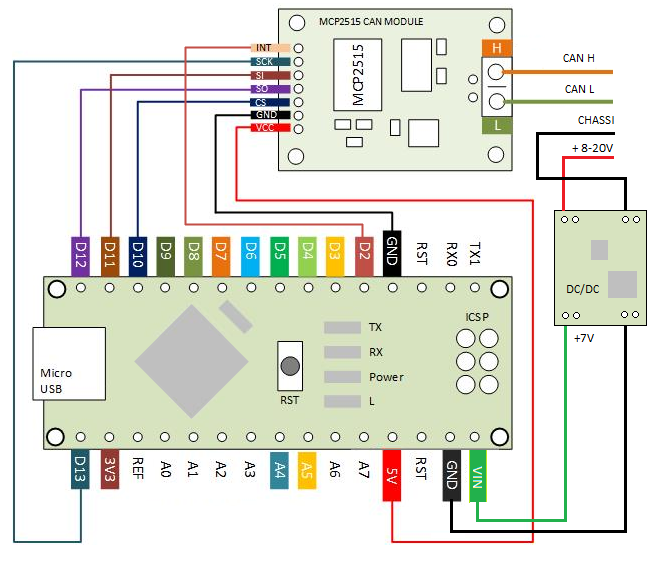
\includegraphics[width=0.45\textwidth]{wiring}
    \caption{Schema van de bedrading van de CAN-controller aan de Arduino \cite{autowp}}
    \label{fig:wiring}
\end{figure}

In het schema in figuur \ref{fig:wiring} is te zien hoe de Arduino de
CAN-controller aan kan sturen. En hoe de Arduino gevoed word met de
\si{12\volt} uit de auto.

%%%%%%%%%%%%%%%%%%%%%%%%%%%%%%%%%%%%%%%%%%%%%%%%%%%%%%%%%%%%%%%%%%%%%%%%
\section{Behuizing}
%%%%%%%%%%%%%%%%%%%%%%%%%%%%%%%%%%%%%%%%%%%%%%%%%%%%%%%%%%%%%%%%%%%%%%%%

\begin{figure}[]
    \centering
    \begin{minipage}{0.45\textwidth}
        \centerline{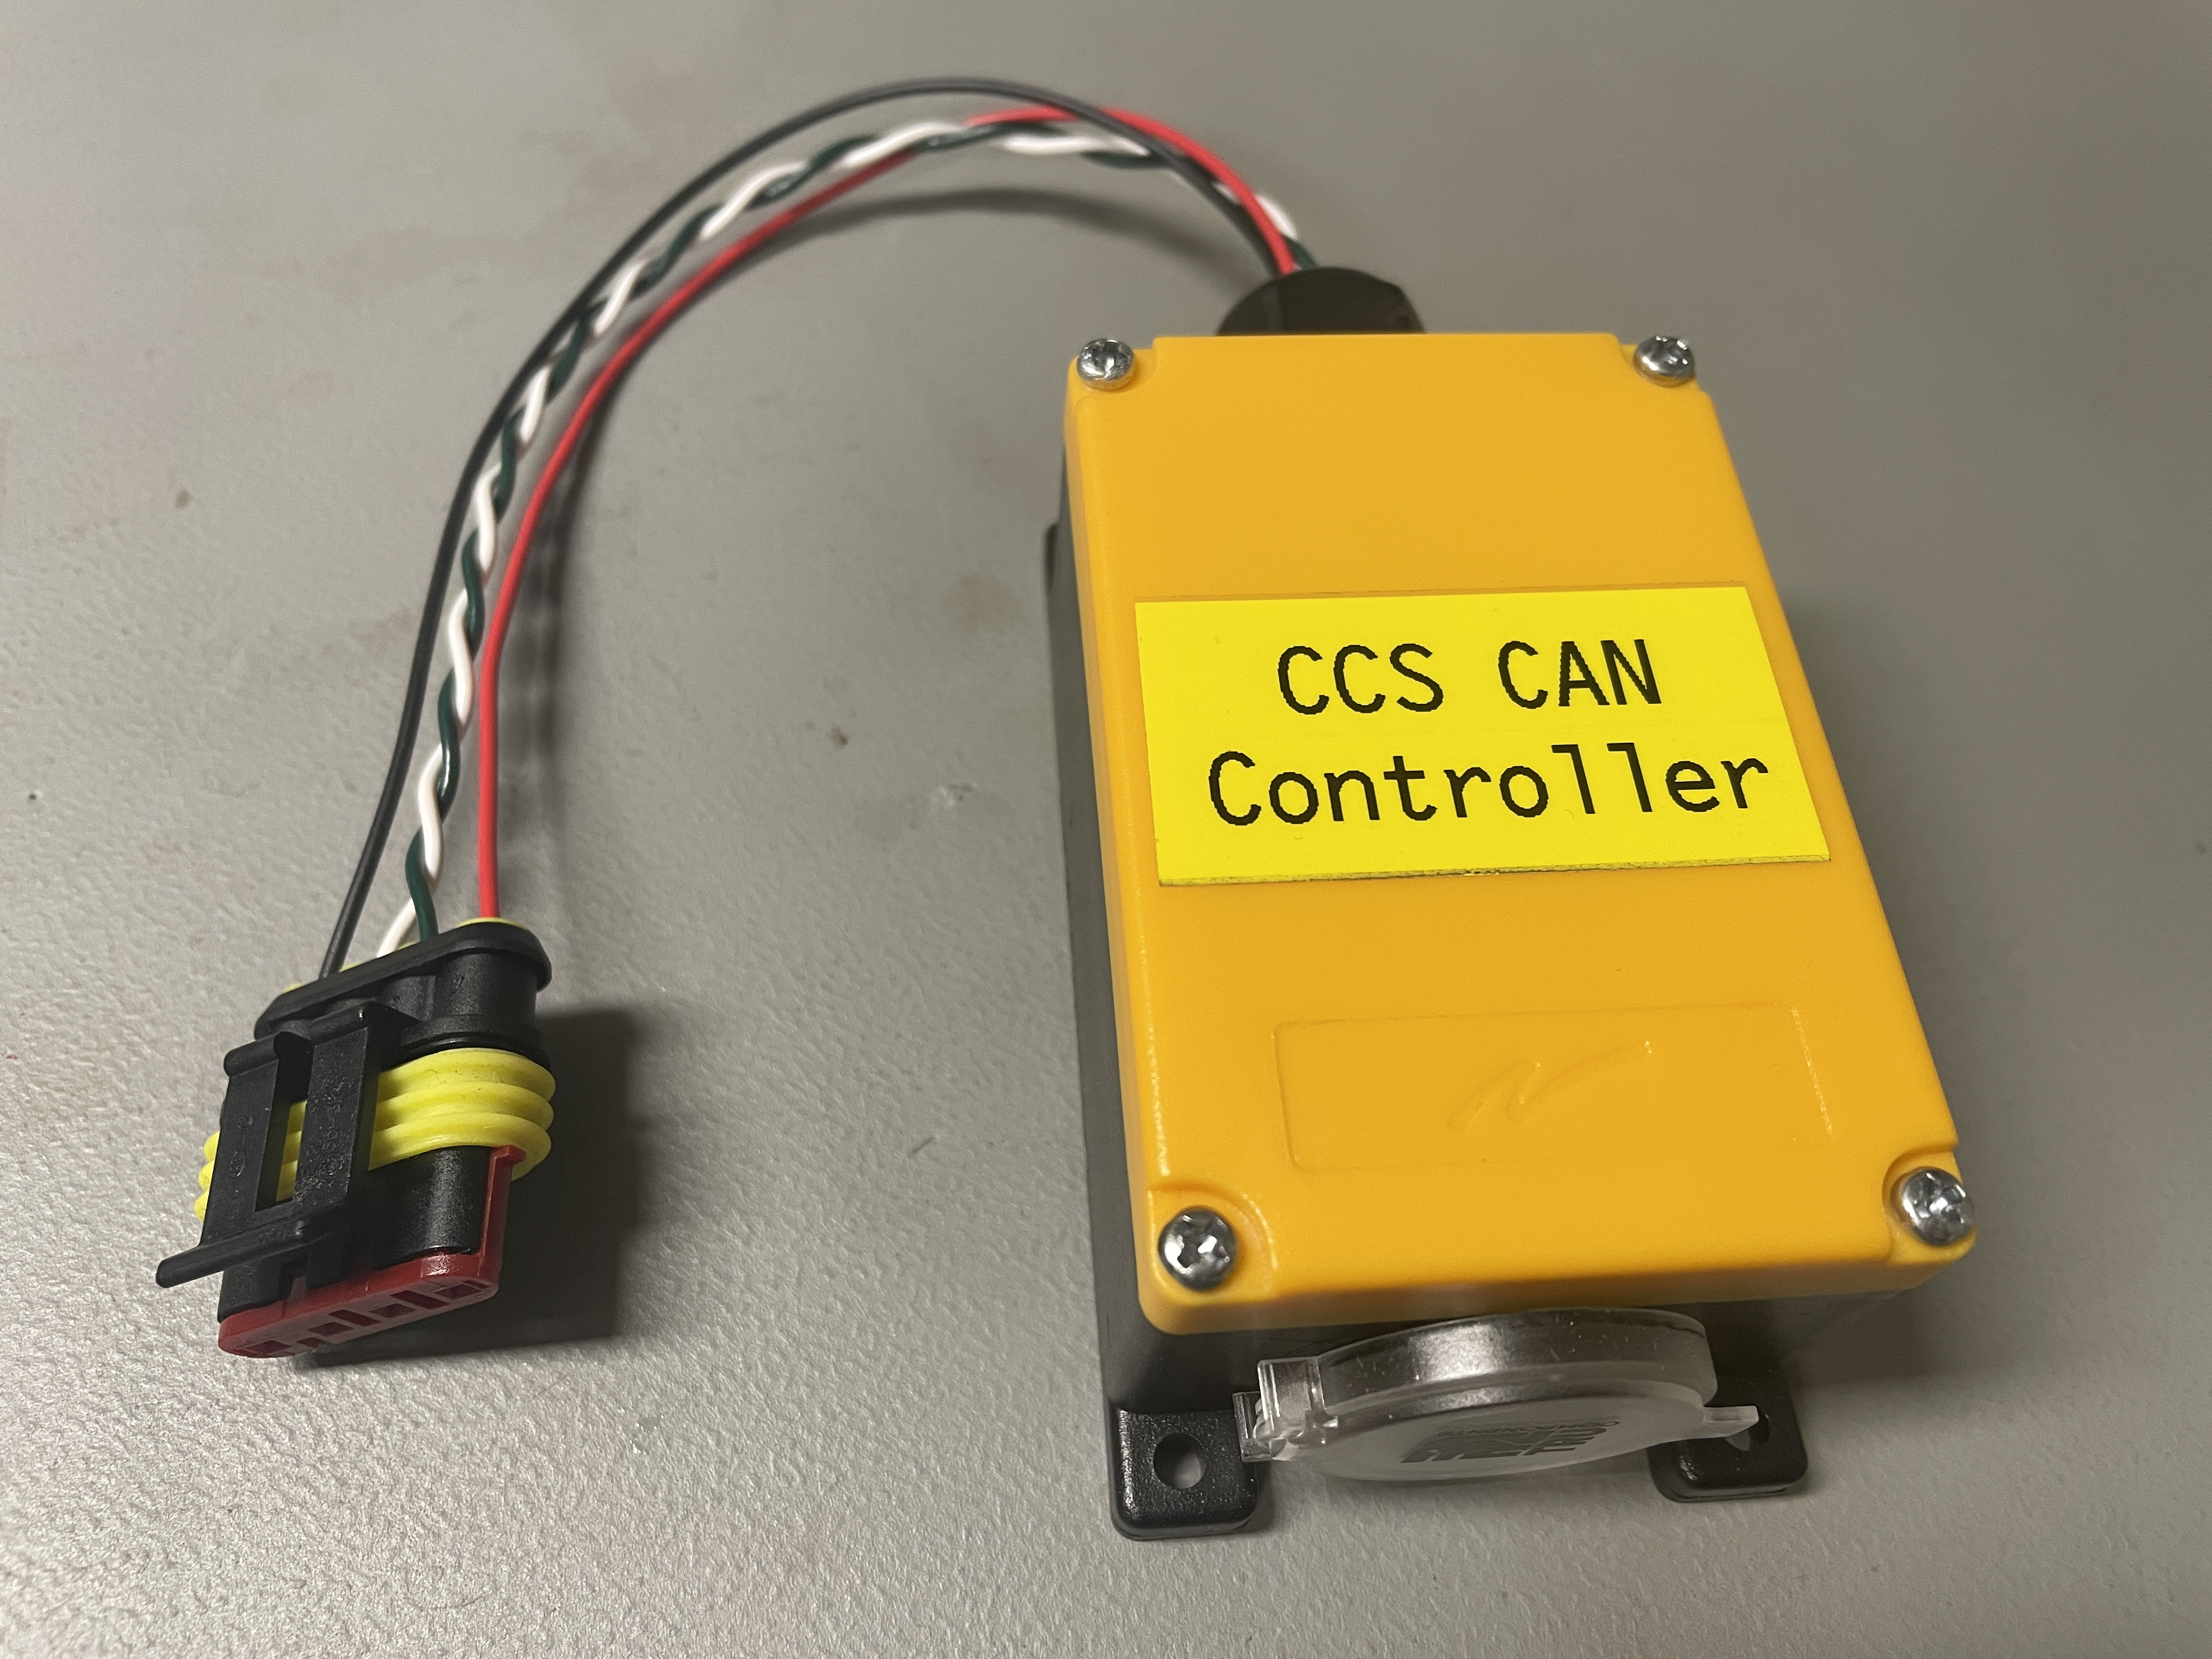
\includegraphics[width=0.9\textwidth]{behuizing}}
        \caption{Behuizing van de CCS CAN controller}
        \label{fig:behuizing}
    \end{minipage}\hfill
    \begin{minipage}{0.45\textwidth}
        \centerline{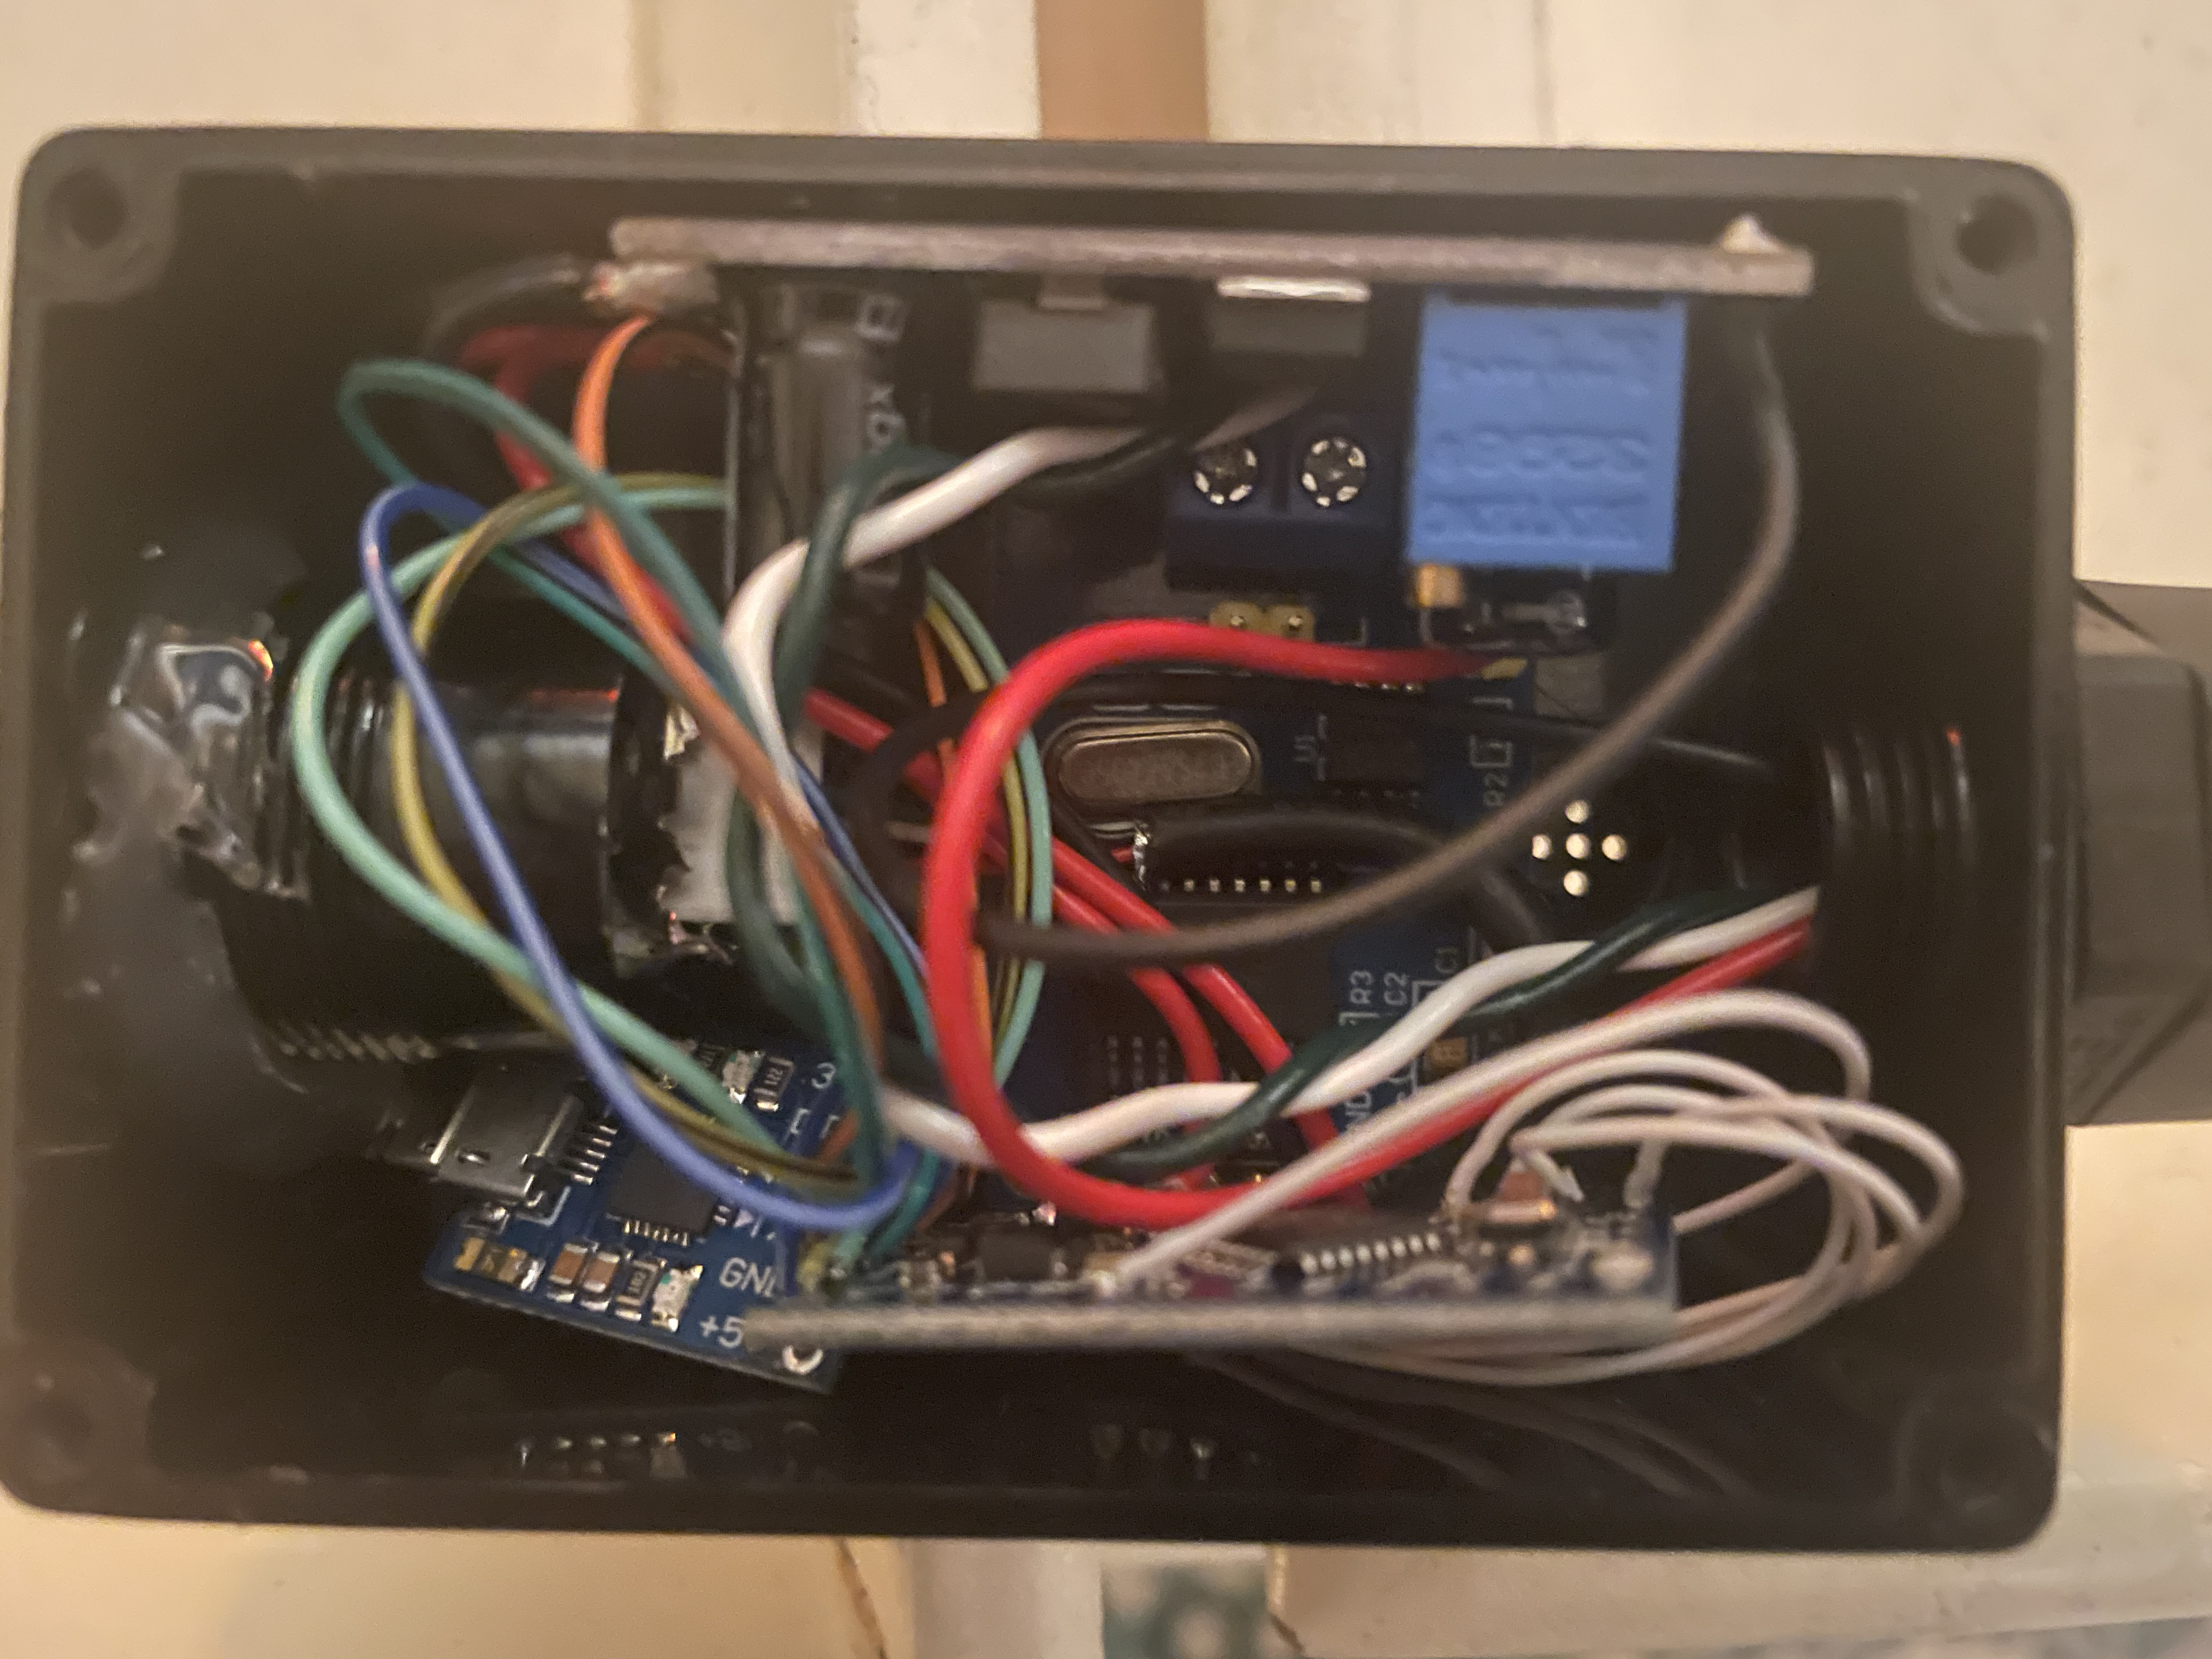
\includegraphics[width=0.9\textwidth]{binnenkant}}
        \caption{Binnenkant van de behuizing}
        \label{fig:binnenkant}
    \end{minipage}
\end{figure}

In figuur \ref{fig:behuizing} is het eindresultaat te zien, een kleine lasdoos
is gebruikt als behuizing, met aan een kant een wartel als doorvoer van de CAN
bus en de \si{12\volt} uit de auto en aan de andere kant een panel mount USB
aansluiting, om de Arduino te kunnen programmeren. In figuur
\ref{fig:binnenkant} is de binnenkant van de behuizing te zien. Het is best
krap aan de binnenkant, maar alles past wel omdat er geen gebruik meer word
gemaakt van headers, maar alle verbindingen zijn direct aan de pcb gesoldeerd.